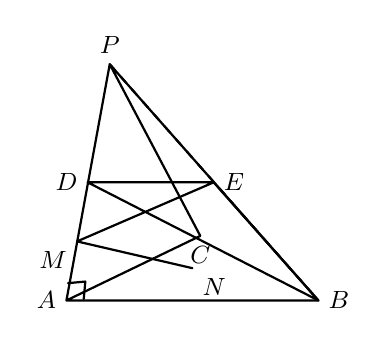
\begin{tikzpicture}[thick,line cap=round,line join=round,
  every node/.style={font=\small}]
  \coordinate (P) at (0,3.0);
  \coordinate (A) at (-.55,0);
  \coordinate (B) at (2.65,0);
  \coordinate (C) at (1.15,.82);
  \coordinate (D) at (-.28,1.5);
  \coordinate (E) at (1.32,1.5);
  \coordinate (N) at (1.05,.41);
  \coordinate (M) at (-.415,.75);
  % Outer pyramid and source-visible internal segments. The right-angle mark
  % is at A, as printed; no unlabelled construction point is added.
  \draw (P)--(A)--(B)--(P) (A)--(C) (P)--(C);
  \draw (B)--(D) (D)--(E) (B)--(E) (E)--(M) (M)--(N);
  \draw[dashed] (P)--(B);
  \draw (A) ++(.22,.02)--++(.02,.22)--++(-.22,-.02);
  \node[above] at (P) {$P$};
  \node[left] at (A) {$A$};
  \node[right] at (B) {$B$};
  \node[below] at (C) {$C$};
  \node[left] at (D) {$D$};
  \node[right] at (E) {$E$};
  \node[below left] at (M) {$M$};
  \node[below right] at (N) {$N$};
\end{tikzpicture}
